%-----------------------------------------------------------------------------
%
%               Template for sigplanconf LaTeX Class
%
% Name:         sigplanconf-template.tex
%
% Purpose:      A template for sigplanconf.cls, which is a LaTeX 2e class
%               file for SIGPLAN conference proceedings.
%
% Guide:        Refer to "Author's Guide to the ACM SIGPLAN Class,"
%               sigplanconf-guide.pdf
%
% Author:       Paul C. Anagnostopoulos
%               Windfall Software
%               978 371-2316
%               paul@windfall.com
%
% Created:      15 February 2005
%
%-----------------------------------------------------------------------------


\documentclass{sigplanconf}

% The following \documentclass options may be useful:

% preprint      Remove this option only once the paper is in final form.
% 10pt          To set in 10-point type instead of 9-point.
% authoryear    To obtain author/year citation style instead of numeric.

% !TEX root =  RefactorToCloud.tex

\usepackage{xspace}
\usepackage{graphicx}
\usepackage{amsmath}
\usepackage{color}
\usepackage[hidelinks]{hyperref}


%\usepackage[english]{babel}
%\usepackage{threeparttable}
%\usepackage{amssymb}
%\setcounter{tocdepth}{3}
%
%\usepackage{multirow}
%\usepackage{url}
%\usepackage{array}
%
%\usepackage{moreverb}
%\usepackage{listings}

%%\usepackage{cite}
%\usepackage{relsize}
%\usepackage{wasysym}
%\usepackage{fancybox}
%\usepackage{balance}
%\usepackage{enumitem}
%\usepackage{lmodern}
%\usepackage{caption}
%\usepackage{epstopdf}
%
%\usepackage[font={bf}, labelfont=bf]{caption}
%\usepackage[font={bf,small},labelfont=bf]{caption}
%\usepackage{datetime}

%\captionsetup[table]{skip=5pt}
%
%\newcommand{\version}[1]{\normalsize{Version #1 - \mydate\today\xspace,\xspace\currenttime}}
%
%\newdateformat{mydate}{\monthname[\THEMONTH]\xspace\THEDAY}
%
%\newcommand{\fixme}[1]{}
\newcommand{\TODO}[1]{\textcolor{magenta}{\textbf{TODO: }#1}}

%\newcommand{\FB}[1]{\textcolor{blue}{\textbf{FEEDBACK: }#1}}
\newcommand{\FB}[1]{{#1}}
%
%\newcommand{\ADD}[1]{\textbf{\textcolor{blue}{#1}}}
%\newcommand{\REMOVE}[1]{\textbf{\textcolor{red}{#1}}}
%
%\newcommand{\mybox}[1]{
%\begin{center}
%\setlength{\fboxsep}{5pt}%
%\Ovalbox{%
%\begin{minipage}{.45\textwidth}
%\begin{center}
%{\it #1} 
%\end{center}
%\end{minipage}}
%\end{center}
%}
%
%
%\lstdefinelanguage{TouchDevelop}
%{
%sensitive=true,
%morekeywords=[1]{
%var, add, if, private, action, returns, for, each, do, where},
%morecomment=[l]{//},
%morecomment=[s]{/*}{*/},
%morecomment=[l][keywordstyle4]{\#},
%morestring=[b]",
%morestring=[b]',
%}
%%
%%\DeclareCaptionFormat{listing}{\rule{\dimexpr\textwidth+17pt\relax}{0.4pt}\par\vskip1pt#1#2#3}
%%\captionsetup[lstlisting]{singlelinecheck=false, margin=0pt, font={sf},labelsep=space,labelfont=bf}
%%\renewcommand\lstlistingname{Code}
%%
%\definecolor{mygreen}{rgb}{0,0.6,0}
%\definecolor{mygray}{rgb}{0.5,0.5,0.5}
%\definecolor{mymauve}{rgb}{0.58,0,0.82}
%%
%\lstset{ %
%%frame=bottom,
%  language=TouchDevelop,                % the language of the code
%  basicstyle=\ttfamily\scriptsize,           % the size of the fonts that are used for the code
%  keywordstyle=\color{blue},
%  commentstyle=\color{mygreen},
%  numberstyle=\tiny\color{mygray}
%  stringstyle=\color{mymauve},
%  rulecolor=\color{black}, 
%  stepnumber=1,                   % the step between two line-numbers. If it's 1, each line 
%  %numbers=left,                   % where to put the line-numbers
%  numberstyle=\scriptsize,  
%  numbersep=5pt,  
%  showspaces=false,               % show spaces adding particular underscores
%  showstringspaces=false,         % underline spaces within strings
%  showtabs=false,                 % show tabs within strings adding particular underscores
%  tabsize=2,                      % sets default tabsize to 2 spaces
%  breaklines=false,                % sets automatic line breaking
%  breakatwhitespace=false,        % sets if automatic breaks should only happen at whitespace
%  belowskip=1pt,
%  aboveskip=2pt
%}
%
%
\newcommand{\codesnippet}[1]{
\begin{lstlisting}#1\end{lstlisting}}
%
%\newcommand{\readme}[1]{\texbf{ReadMe: }#1}
%
%\newcommand{\etal}{\emph{et~al}.~}
%\newcommand{\Comment}[1]{}%\textbf{\textsl{$\langle\!\langle$#1$\rangle\!\rangle$}}}
%\newcommand{\spacedinlineheader}[1]{\vspace{1.5 mm} \noindent \textbf{#1}}
%\newcommand{\Space}[1]{}


\newcommand{\numScripts}{116\xspace}
\newcommand{\numManual}{20\xspace}
\newcommand{\numFormative}{four\xspace}
\newcommand{\MT}{\begin{small}\textsc{Mileage Tracker}\end{small}\xspace}
\newcommand{\numTransformations}{2722\xspace}
\newcommand{\percentRefactored}{94\%\xspace}
%\newcommand{\TD}{TouchDevelop\xspace}
\newcommand{\TD}{\textsf{touch\textbf{develop}}\xspace}
\newcommand{\NC}{\code{Number Collection}\xspace}
\newcommand{\CDT}{\code{Cloud Data Table}\xspace}

\newcommand{\POne}{\textbf{(P1)}\xspace}
\newcommand{\PTwo}{\textbf{(P2)}\xspace}

\newcommand{\code}[1]{\begin{small}\texttt{#1}\end{small}}
%\newcommand{\URL}[1]{\begin{footnotesize}\url{#1}\end{footnotesize}}


\newcommand{\tool}{\begin{small}\textsc{Cloudifyer}\end{small}\xspace}



%\newcommand{\RQOne}{\textbf{RQ1:} How do developers use asynchronous programming?\xspace}
%
%\newcommand{\MisuseOne}{\subParagraph{(1) Fire \& Forget methods:}\xspace}








%Are they \textbf{safer} than manual approach?\xspace}
%Do they improve \textbf{code quality}?\xspace}

%\newcommand{\subParagraph}[1]{\textbf{\emph{#1}}}
\newcommand{\myParagraph}[1]{\noindent \textbf{#1}}








\usepackage{listings}
\usepackage{color}
\usepackage{xspace}
\usepackage{alltt}

 \usepackage{multirow} 
 \usepackage{rotating}
%%%%%%%%%%%%%%%%%%%%%%%%%%%%%%%%%%%%%%%%%%%%%%%%%%%%%%%%%%%%%%%%
%%%% THIS BELOW COPIED FROM vkuncak/doc/vmcai09/defs.tex
\definecolor{gray}{RGB}{211,211,211}
\newcommand{\jbasicstyle}{\scriptsize\sffamily}%\footnotesize}
\newcommand{\textcode}[1]{{#1}} % with current font \sf and \tt look ugly
\newcommand{\jnumberstyle}{\tiny}
\newcommand{\Hilight}{\makebox[0pt][l]{\color{gray}\rule[-3pt]{0.80\linewidth}{9pt}}}
\newcommand{\CodeIn}[1]{{\small\texttt{#1}}}

\newcommand{\codex}[1]{{\smaller\texttt{#1}}\xspace}

\newcommand{\tilted}[1]{\begin{turn}{75}#1\end{turn}}

\lstdefinelanguage{pseudo}
 {
%alsoletter={<>:=},
  morekeywords={int,boolean,new,continue,enum,
                void,if,else,while,return,for,foreach,in,assert,assume,false,true,class,static,import,
                ignoreIf,getInt,getAny,getNew,getExisting,getBoolean,force,concrete,Susp,
                getInt,getAny,getNew,getBoolean,force,concrete,Susp,max,min,ObjectPool,
                implements,interface,public,double,synchronized,final,
                proc,@Event,@Schedule,extends,case,sleep,waitForTick,assertTick,instanceof},
  keywordstyle=\bfseries,
  lineskip=-0.1em,
%  numbers=left,
  numbers=none,
  numberstyle=\jnumberstyle,
  numbersep=4pt,
%  basicstyle=\scriptsize,
  basicstyle=\jbasicstyle,
  breaklines=true,
  breakautoindent=true,
  tabsize=2,
%  columns=fixed,
%  columns=flexible,
  columns=fullflexible,
%  morecomment=*[s][\textsl]{/*:}{*/},
  morecomment=*[l][\textsl]{//},
%  morecomment=*[s][\jahobform]{"}{"},
  mathescape=true,
%  escapeinside=<>,
%  escapebegin={\begin{isakeyword}},
%  escapeend={\end{isakeyword}}
%  caption={},
%  label={},
}
\newcommand{\MyParagraph}[1]{\noindent \textbf{#1}}
\newenvironment{CodeOut}{\begin{scriptsize}}{\end{scriptsize}}



\newcommand{\vertbar}{vertBar\xspace}




\newcommand{\NumProjects}{9\xspace}
\newcommand{\NumSLOCReduced}{2213\xspace}
\newcommand{\NumOperationsInferred}{2681\xspace}
\newcommand{\NumChainsInferred}{1709\xspace}
\newcommand{\NumSLOCChangedAnon}{3707\xspace}
\newcommand{\NumSLOCChangedFor}{12313\xspace}
\newcommand{\NumSLOCChanged}{16020\xspace}


\usepackage{subfigure}
\usepackage{graphicx}
\usepackage{algorithm}
\usepackage{algpseudocode}
\usepackage{url}
\usepackage{footnote}
%\usepackage{biblatex}
%\usepackage{natbib}
\usepackage{balance}

\usepackage{float}
\restylefloat{table}





%\usepackage{hyperref}
%\pagenumbering{arabic}

\begin{document}

\special{papersize=8.5in,11in}
\setlength{\pdfpageheight}{\paperheight}
\setlength{\pdfpagewidth}{\paperwidth}

\conferenceinfo{CONF 'yy}{Month d--d, 20yy, City, ST, Country} 
\copyrightyear{20yy} 
\copyrightdata{978-1-nnnn-nnnn-n/yy/mm} 
\doi{nnnnnnn.nnnnnnn}

% Uncomment one of the following two, if you are not going for the 
% traditional copyright transfer agreement.

%\exclusivelicense                % ACM gets exclusive license to publish, 
                                  % you retain copyright

%\permissiontopublish             % ACM gets nonexclusive license to publish
                                  % (paid open-access papers, 
                                  % short abstracts)

\titlebanner{banner above paper title}        % These are ignored unless
\preprintfooter{short description of paper}   % 'preprint' option specified.

\title{Refactoring towards Cloud-enabled Multiuser Mobile Apps}

\authorinfo{Arpit Christi }
           {Oregon State University}
           {chrsitia@eecs.oregonstate.edu}
\authorinfo{Michael Hilton}
           {Oregon State University}
           {hiltonm@eecs.oregonstate.edu}
\authorinfo{Danny Dig}
           {Oregon State University}
           {digd@eecs.oregonstate.edu}
\authorinfo{Michal Moskal}
           {Microsoft Research}
           {Michal.Moskal@microsoft.com}
\authorinfo{Sebastian Burckhardt}
           {Microsoft Research}
           {sburckha@microsoft.com}
\authorinfo{Nikolai Tillmann}
           {Microsoft Research}
           {nikolait@microsoft.com}
\maketitle


\begin{abstract}
Cloud computing has become a great tool for many developers to use, with many benefits, especially in mobile development.  However, adding cloud functionality to an existing app can be difficult and time-consuming. We present \tool, a tool that can automatically refractor \emph{local} data structures into \emph{cloud} data structures on the TouchDevelop platform.  As this platform targets students and hobbyist programmers, lowering the barrier of entry to using the cloud is imperative.  

\end{abstract}


\section{Introduction}

% mobile is everywhere. mobile cloud computing can make it better. Examples of multiuser apps
Mobile apps have gained significant popularity in the recent years. According to Gartner~\cite{Gartner}, by 2016 more than 300 billion apps will be downloaded annually. The cloud has amplified the utility of mobile devices by providing additional computing power and storage, which translate into improved battery life~\cite{Chen:2012:CCO:2310096.2310228}, security~\cite{Oberheide:2008:VIS:1622103.1629656}, bandwidth utilization~\cite{Vemulapalli:2013:PSD:2492348.2492353}, location awareness~\cite{kansal2013latency}. In this paper we are focusing on another killer feature enabled by the cloud: the ability to develop rich, multiuser apps. Examples abound from domains such as social networking (e.g., Facebook, Twitter), multiplayer games, collaborative data collection (e.g., Citizen Science~\cite{cohn2008citizen}). 

% What's broken: advanced expertise, infrastructure, multiple languages
To take advantage of the benefits of the cloud, app developers face a high entry barrier. They need expertise on many topics: communication protocols (e.g., web services, REST, SOAP, etc.), data storage (e.g., Amazon S3, Microsoft SkyDrive, etc.), databases, cloud infrastructure (e.g., Amazon EC2, Windows Azure, etc.),  programming or scripting languages. Similarly, converting a single into a multiuser app has a high entry barrier: they need to determine the candidate data structures and methods that operate on data structures and move them to the cloud. Currently, this process is manual, time consuming, and error prone~\cite{khan2013survey}.

% In this paper we want to lower the entry barrier for developers, so that even hobbyists and beginner mobile app devs. Thus, TouchDevelop + Refactoring
In this paper we are lowering the entry barrier to allow even hobbyists and beginner app developers to use the cloud. Thus, we are targetting TouchDevelop~\cite{Tillmann2011TPC20482372048245}, a programming environment and language developed by Microsoft Research to write apps \emph{on} mobile devices for mobile devices. We are employing automated refactoring techniques to convert local data structures into cloud data structures.

% Intro to TouchDevelop and its cloud datatype
TouchDevelop introduced specialized cloud data types~\cite{burckhardt2012cloud} that provide an abstraction layer over web service implementation, communication protocols, and storage.  In order to make the app responsive, even when the connection to the server is unavailable, cloud data types provide both local copies of the data as well as eventually consistent sharable cloud storage. This paradigm allows programmers to use cloud types in a similar manner to local data structures, but to also enjoy the benefits of the cloud.

% Our formative study to learn about refactorings from single to multi-user apps. refactorings for data structures
In this paper we present the results of our formative study to convert single to multi-user apps. We used \numFormative publicly available, single-user TouchDevelop apps (two productivity tools and one game) and manually converted them into multi-user apps. Thus we discovered four conversion steps: (i) identify local data structures that need to be shared between multiple users, (ii) for each identified local data structure add a new cloud data structure, (iii) replace local data structure API calls with cloud API calls, (iv) initialize the cloud data structures. Not all these steps can be automated; some (e.g., identifying data structures that need to be shared) require domain knowledge which is best provided by the app developer. 

% Automated refactoring based on these lessons, why do we need refactoring support.
Using the lessons that we learned from the formative study, we designed and implemented a refactoring tool, \tool, to automate the conversion of local \NC{} into \code{Cloud Data Table}, and to transform the API calls. We selected this refactoring because its manual application is 
challenging: the developer needs to map a 1-dimensional, horizontal data layout (as in \code{Collection}) into a 2-dimensional data layout (as in \code{Table}).
The difference is not only in the names of the APIs, but also in the cardinality of the mapping.
Sometimes the mapping is 1-to-1 (e.g., \code{count} is the same in both data structure), other times the mapping is 1-to-many (e.g., \code{insert at} from \code{Collection} is transformed into a sequence of 3 operators from \code{Table}). In addition, sometimes there is no mapping, in which case it requires creating custom functions to achieve the same computation. For example, \code{Collection->max} needs to be converted into a custom function that iterates atomically over the elements of the \code{Table}. Such transformations can not be performed by a find-and-replace tool.

% Contributions
This paper makes the following contributions:
\begin{itemize}
\item{\textbf{Idea:}} To the best of our knowledge, we are the first to enable hobbyists and beginner programmers to tap into the power of the mobile cloud
computing through the use of refactoring techniques.

\item{\textbf{Formative Study:}} We have conducted a formative study on \numFormative real-world apps to learn what transformations are needed to convert single to multi-user mobile apps. 

\item{\textbf{Tool:}} We have designed and implemented the analysis and transformation algorithms to refactor \emph{local} data structures into \emph{cloud} data structures on the TouchDevelop platform. 

\item{\textbf{Evaluation:}} We have evaluated our tool, \tool, on a corpus of \numScripts mobile apps, resulting in \numTransformations transformations. The results show (i) that the refactoring is widely \emph{applicable}: \percentRefactored of the candidate local \code{Collection}s were successfully refactored into \code{Cloud Data Table}. Second, \tool saves human effort: on average it took 9 seconds for each performed refactoring. Third, \tool is  
\emph{accurate}: 100\% of the applied transformations are correct, and the tool correctly identified 95\% of all necessary transformations.  
\end{itemize}

%\Comment{eat this line}
\section{Background on TouchDevelop Cloud Data Types}


\section{Formative Study}

%describe the applications
We selected \numFormative apps from the \TD script bazaar for our formative study. We converted them from single-user to multi-user apps. In this section we describe the script's behavior, the process to convert them, as well as the changes we needed to make.

The first app we selected was \MT, which is publicly available with the script id of~\cite{MileageTracker}.  Mileage Tracker is an app that records and calculates fuel usage in Miles per Gallon (MPG) and displays how it changes over time. We converted Milage Tracker into a multi-user app, such that multiple family members using the same family car can collect the fuel usage even across multiple devices.

Business Manager+~\cite{BusinessManager} is an app to track of business contacts.  We converted it into a multi-user app so that business colleagues can share their contact list with others.

CliffHangers~\cite{CliffHangers} is a clone of the popular game ``hangman."  The player is presented with a series of blanks, and they must guess the letters that fill in the blanks to make a word.  The player has a limited number of guesses, and if they cannot guess the word before they reach the limit, they loose the game.  We converted it into a multi-player game so that two players can collaboratively work together on separate devices to guess the word.

MyAssignment~\cite{MyAssignments} is an app for students to track their class assignments or projects.  A single user can input information about projects, progress, due dates, etc.  We converted into a multi-user app so that multiple students can collaborate on class assignments.

After converting these apps, we ran them with multiple users to verify that in fact the apps work correctly. 

%describe the process with the four steps
Based on the lessons we learned from converting these \numFormative apps, we designed a process to convert  a single to a multi-user app.  Our process consists of four steps:   
\begin{enumerate}
\item Identify data that needs to be shared between users

\item Create new Cloud Data Structures to hold the shared data

\item Replace the local usage with cloud usage for the shared data

\item Initialize Cloud Data
\end{enumerate}

Next we will illustrate these steps using the \MT app.  In step 1 we identified the data that needed to be shared: 
(i) the \code{MilageRecord} is a collection of numbers that holds the Miles Per Gallon for the past usage consumption, 
(ii) \code{MaximumRecordEntries} is a number that determines how many records should be stored, 
(iii) \code{UseUSUnits} is a boolean that stores the preference between metric or imperial units.
   
To illustrate step 2, let us consider one of the shared data structures, the \code{MilageRecord} collection. 
We created a new \code{Cloud Data Table} named \code{MileageRecordTable} to hold the data. Notice that the
original data is stored in a one-dimensional data structure, whereas the \code{Cloud Data Table} is a two-dimensional data 
structure.

In step 3 we replaced all the uses of the local \code{MilageRecord} with uses of \code{MileageRecordTable}. 

In step 4 we initialized  \code{MileageRecordTable}. 
Since the data is now persistent on the cloud, we need to change the initialization code from 
eager to lazy in order to avoid erasing all the data every time the app is launched.  
In addition, we need to make a choice between using the cloud (i) as a backup for the data for one user across multiple devices(``just me session'') versus (ii) to enable collaboration between multiple users across multiple devices (``everyone session'').

%STEP ONE AND 4 REQUIRE DOMAIN KNOWLEDGE
Notice that steps 1 and 4 require domain knowledge in order to choose and refine the proper end-user experience.  
 
% NEXT WE DESCRIBE THREE REFACTORINGS
Based on the type of the input, local data that we needed to migrate to cloud, we have identified three kinds of refactorings. Each refactoring can be performed using the general steps that we identified above. First, we refactored primitive data 
types into the corresponding cloud-enabled primitive type (e.g., from \code{Number} to \code{Cloud Number}).
Second, we refactored local \code{Data Table} into \code{Cloud Data Table}. Third, we refactored local \code{Collection}
into \code{Cloud Data Table}.

When carrying out the refactorings, we noticed that steps 1 and 4 are hard to automate as they require understanding the original program and the desired end-user experience. Steps 2 and 3 have different degrees of complexity. 
The first two kinds of refactorings  are trivial because there is a perfect match between the local data and the cloud data type, so the change is as simple as prepending the keyword \code{Cloud} to the variable declaration. 

The third kind of refactoring is non-trivial: it requires changing the program from using a flat, one-dimensional \code{Collection} to a two-dimensional \code{Cloud Data Table}. The APIs are different enough, so that sometimes we needed to map one function call from \code{Collection} into a sequence of calls from \code{Table}, whereas other times we had to augment the API by writing new functions. 
For these reasons, we automated the refactoring. 

Table~\ref{tab:refactoringsFormative} lists the total number of refactorings that we applied as part of our formative study.

\begin{table}[htdp]

\begin{center}
\begin{tabular}{|c|c|c|c|}
\hline
App  & Primitive to  & Local Table to   & Collection to  \\
 Name &  Cloud  &  Cloud Table  & Cloud \\
\hline
MileageTracker & 2 & 0 & 1\\
\hline
Buisness Manager+ & 0 & 0 & 5\\
\hline
CliffHangers & 8 & 0 & 2\\
\hline
My Assignments & 0 & 1 & 0\\
\hline
\hline
Total & 10 & 1  & 8 \\
\hline
\end{tabular}
\end{center}
\nocaptionrule
\caption{Total number of refactorings}
\label{tab:refactoringsFormative}
\end{table}%



%describe the refactoring targets with tables to show frequency

\section{Automated Refactoring}

\begin{figure*}
   \centering
    \mbox{
      \lstset{
	  language=Java, numbers=left, keywordstyle=\color{blue}, commentstyle=\color{red}, stringstyle=\color{black}, basicstyle=\scriptsize, tabsize = 2, moredelim=[is][\underbar]{_}{_}
      }
      \subfigure[before]{
      \lstinputlisting[]{src/in/TouchDevelopBefore.txt}
      \label{fig:aicOverload}
      }
      \hspace{0.2in}
      \subfigure[after]{
      \lstinputlisting[]{src/out/TouchDevelopAfter.txt}
      \label{fig:lambdaOverload}
      }
    }
    \caption{Selected code from Mileage Tracker app}
    \label{fig:anonCornerCase2}
\end{figure*}


\section{Evaluation}

\section{Related Work}

\section{Conclusion}



\section{Motivating Example}
\label{sec:motivatingExample}
In this section we introduce a motivating example for refactoring data structures to the cloud.   Consider a program called Mileage Tracker that allows the user to store their milage so that they can be aware of their fuel usage.  The user can input how much gas was needed to fill his tank, as well as the miles driven since the last fill up.  This allows the application to be able to calculate what was the miles per gallon since the last fill up.  The script will store this information and allow the user to view their fuel usage over time.  This application was written before the introduction of cloud data to the TouchDevelop platform, and so the way that the application was developed, the data was being stored locally in a local data structure.  The developer did check the option which preserves the values of the data structure across multiple runs, so as long as user uses same device, he will have up to date information regarding its mileage usage.  However, the script cannot work across multiple devices which does not support the ability for multiple family members using the same family car to share their information effectively.


\subsection{Goals of Refactoring to Cloud}
The developer of the MPG tracking application would like to take advantage of cloud functionality.  Specifically, the developer would like to enable the users to be able to access their data on multiple devices and see the same data. The developer would also like to enable social, collaborative features such as allowing users to share their MPG values with other users of the app.

This program was written before the introduction of the cloud API's to the TouchDevelop language.  The program does not use any cloud data types, and all data is stored locally.

Before the introduction of the cloud data types, the developer could select the "save between script runs" option for local data, which would persist the data structures across multiple runs of the script.  This approach has several limitations which significantly reduce the usefulness of the application to the end user.  One of the major limitations of this approach is that the information can not be synced between devices.  The user would only be allowed to track their MPG's on one single device.  This poses a problem if the user would like to upgrade their device,or if there phone was lost or broken.   Also, this approach will not work if there are multiple drivers of the vehicle, and they would like to be able to collaborate on tracking their fuel efficiency.  However, this would not be possible using the local data structure.


  
\subsection{Problem}
If the application had been developed using the TouchDevelop table data structure, converting to a cloud table is a trivial operation.  It is as simple as selecting the table object and changing the type to cloud table.  The refactoring becomes non-trivial if the user was using another data structure, such as a collection. A TouchDevelop collection is a data structure that consists of a collection of any type of object that TouchDevelop supports.  This could be a primitive type such as Number or String, or it could be something as complex as a Camera object, or a Map object.  The difficulty in refactoring an existing collection into a cloud data structure arises in the need to convert into a cloud table.  The methods that collection provides and the methods that cloud table provides have some overlap, but are not consistent.  In addition, there are methods for \NC{} that have no counterpart for cloud table, i.e. avg.  Table~\ref{tab:mappingTable} shows the operations that are available for \NC{}s, as well as the corresponding operations for cloud table, if they exist.  We have categorized the type of transformation that will be necessary to transform every possible collection operation into a cloud table operations.  We will describe how we perform these transformations Section~\ref{sec:Refactoring}.

\begin{table*}[htb!]
\centering
\begin{center}
\begin{tabular}{|c|c|c|}
 \hline
Number Collection Operations & Cloud Table Operations & Transformation Type\\
 \hline
  \hline
\code{add} & \code{add row} & Indirect \\ 
\hline
\code{at} & \code{row at} & Indirect \\
\hline
\code{add many} & NONE & Function \\
\hline
\code{avg} & NONE & Function \\
\hline
\code{clear} & \code{clear} & Direct \\
\hline
\code{contains} & NONE & Function \\
\hline
\code{count} & \code{count} & Direct \\
\hline
\code{index of} &NONE  & Function \\
\hline
\code{insert at} & \code{row at$\rightarrow$value} & Indirect \\
\hline
\code{max} &NONE  & Function \\
\hline
\code{min} & NONE & Function \\
\hline
\code{post to wall} & \code{post to wall} & direct \\
\hline
\code{random} &NONE  & Function \\
\hline
\code{remove}  & NONE & Function \\
\hline
\code{remove at} & \code{row at$\rightarrow$deleteRow} & Indirect \\
\hline
\code{reverse} &NONE  & Function \\
\hline
\code{set at} & \code{row at$\rightarrow$valueName} & Indirect \\
\hline
\code{sort} & NONE & Function \\
\hline
\code{sum} & NONE & Function \\
\hline

\end{tabular}
\nocaptionrule
\caption{Table with the Number Collection API's and corresponding Cloud Table Operations}
\label{tab:mappingTable}
\end{center}
\end{table*}%


\section{TouchDevelop}
\label{sec:TouchDevelop}
In this section we provide a brief overview of the TouchDevelop language, as well as some more discussion on how cloud data types are implemented.

\subsubsection{Cloud Data Types}
The cloud types implemented in TouchDevelop include both simple types, cloud integers, cloud strings, as well as the structured types of cloud arrays and cloud entities.   The only way that these cloud types are exposed to developers is as cloud tables and cloud indexes.  The cloud table can be used in a similar manner as the local table data structure.  However, when a developer uses the cloud table, they also get an eventually consistent cloud version and the option to share the data across multiple users.

If the developer wished to take advantage of the cloud features for primitive data, they must encapsulate them into a table first.  Table~\ref{table:supportedTypes} lists the types of primitives that are allowed as column types of the cloud table.

\begin{table*}[htb!]
\begin{center}
\begin{tabular}{lcl}
  Supported Cloud \\
  Table Types  \\
   \hline
Boolean  \\
Number \\
String  \\
DateTime  \\
Location  \\
User  \\
\end{tabular}
\nocaptionrule
\caption{Supported Types}
\label{table:supportedTypes}
\end{center}
\end{table*}%



\subsubsection{sessions}
There are two different types of cloud sessions that are offered by TouchDevelop.  There is the default session, called the "just-me" session as well as the "everyone" session.  \subsubsection{just-me session}
The "just-me" session is meant to share data between all devices by the same user running the same script.  Other users cannot connect to this session.  When the MPG script is refactored to use the just-me session, the user will now have the opportunity to see all of their data regardless of which device they are on. This allows the user to have the application installed on their phone and tablet and to share the data across each. 

\subsubsection{everyone session}
The "everyone" session creates a session that everyone running the script can connect to.  All users of the script will see the same data.  For the MPG example, the everyone session would allow users to see the MPG statistics of a community of users.  All users would add their MPG data to the common table, and the statistics that they would see would be for the entire community.  For example, when they see the average MPG, it would be the AVG for all the users of the script.



  
\section{DataStructure to Cloud REFACTORING}
\label{sec:Refactoring}
This section presents the data structure to cloud refactoring.  We explain \tool's workflow, as well as the three types of transformations that we have identified that are necessary for the refactoring. 

\subsection{Workflow}
\tool is written in TouchDevelop, and can be run using the TouchDevelop platform.  Once it is run, the user is presented with a picker to choose which script to refactor.  This must be a script that is saved for that user, but any public script can be saved as your own script. When the user selects which script they wish to refactor, they are presented with all \NC{}s that are a part of this script.  The user can then choose which \NC{} they wish to refactor by typing in the name into a standard TouchDevelop wall prompt box. Once the user has typed in the name and clicked the ``ok'' button, the tool will automatically refactor all the calls to the selected \NC{}, and then present some output to the user, which includes how many of each type of transformation were performed, as well as the total time required to complete the refactoring. 


\subsection{Algorithm}
We describe the algorithm that is used by the refactoring engine to refactor TouchDevelop scripts.   

Step 1: Create a new Cloud Data structure that transformations will use and add it to the script.

Step 2: Traverse through the script and find candidate statements for refactoring.

Step 3: Refactor local data structure statements into corresponding cloud data structure statements.

To explain our algorithm, we will walkthrough the refactoring of a TouchDevelop script, BlockY World.  BlockY World is a game where our hero must find his way through a maze of blocks, while also being able to move blocks to change the environment around him.  BlockY World uses multiple \NC{}s named \texttt{stats}, \texttt{spestats} and \texttt{zones}. For our further discussion of algorithm, we assume that user has selected \texttt{spestats} as the \NC{} to refactor. In step 1, a cloud data type is created and injected by \tool into the BlockY World script.  A new cloud data table is added for every refactoring to avoid conflicts if there are more then one refactoring per script. Then a column will be added to the table with the same name as the \NC{} that is being refactored.  For \texttt{spestats}, the tool will produce a cloud data table with a single column whose data type is number and who's column name is \texttt{spestats}.  In step 2, TouchDevelop's JSON AST tree representation is used to traverse script's AST. If any references to selected collection to refactor is found, the tool marks it as a candidate statement to refactor.  In step 3, each of the candidate statement is then transformed into individual new statement that replace the call to the \NC{} with a the corresponding cloud data action. 

\subsection{Transformations}
There are several categories of transformations that are needed to transform local data structures to cloud data structures.  


\subsubsection{Direct Transformations}
These are the transformations where both the \NC{} and the cloud table have the same action.  For example, both have an action "post to wall" which will, as expected, post to the scripts wall.  This is the simplest of the transformations, as all that is needed to do is replace the object that the action is being called on.  Figure~\ref{fig:numCol_postToWall} shows a line of TouchDevelop code that posts to the wall a \NC{} that is stored in the global variable named \texttt{MileageRecord}.


\begin{figure}[htbp!]
\begin{center}
\texttt{MileageRecord $\rightarrow$ post to wall}

\end{center}
\nocaptionrule
\caption{post to wall before transformation}
\label{fig:numCol_postToWall}
\end{figure}

\begin{figure}[htbp!]
\begin{center}
\texttt{Cloud Data table $\rightarrow$ post to wall}
\nocaptionrule
\caption{post to wall after transformation}
\label{fig:CloudTable_postToWall}
\end{center}
\end{figure}

Figure~\ref{fig:CloudTable_postToWall}  shows the same line of code after it has been transformed by our algorithm.  Now the cloud data table is being posted to the wall.




\subsubsection{Indirect Transformations}
The indirect transformations are slightly more complex then the direct transformations.  The indirect transformation is when there are two actions that have similar behavior, but different names.  For example, \texttt{add}, which adds to a \NC{}, and \texttt{add row} which adds to a cloud data table.  Consider the case where the user of the previous example would like to add the current mileage to the list that stores all the past mileages.  In order to add it to a \NC{}, the developer would have to use the \texttt{add} operator.  This is shown in Figure~\ref{fig:numCol_Add}.

\begin{figure}[htbp!]
\begin{center}
\texttt{MileageRecord $\rightarrow$ add(Mileage)}
\nocaptionrule
\caption{add action before transformation}
\label{fig:numCol_Add}
\end{center}
\end{figure}
\begin{figure}[htbp!]
\begin{center}
\texttt{Cloud Data table $\rightarrow$ add row $\rightarrow$ MileageRecord := Mileage}
\nocaptionrule
\caption{add action after transformation}
\label{fig:CloudTable_Add}
\end{center}
\end{figure}

Figure~\ref{fig:CloudTable_Add} shows the same line of code after it has been transformed by  \tool.  Now the actions are operating on a cloud data table.  Since each element in the \NC{} is being mapped to a row in the cloud data table, before the number can be added a new row must be added to the table.  TouchDevelop offers the ability to chain functions together, so we can chain the add and assignment operators.  In the same line of code we can add a new row to the table, as well as set the value as the current Mileage that we wish to store.


\subsubsection{Custom Function Transformations}
The third type of transformation we have implemented is custom function transformations.  These are needed when there is no action in Cloud Table that will achieve the same functionality as the action that exits in  \NC{}. For example, the developer of the mileage tracker would like to calculate the average across all the sessions of the app.  The \texttt{avg} action will return the average of all the numbers in the \NC{}.  In order to transform a \NC{}s that contain this action, we inject a custom function into the code that provides the same behavior as the \texttt{avg} action.  Then we can transform a call from the TouchDevelop API to a call to our custom function.  Figure~\ref{fig:numCol_avg} shows a line of source code where the \texttt{avg} action is being called, and then the returned value is being stored in a local variable \texttt{avgMielage}.


\begin{figure}[htbp!]
\begin{center}
\texttt{var avgMileage := MileageRecord $\rightarrow$ avg}
\nocaptionrule
\caption{avg action before transformation}
\label{fig:numCol_avg}
\end{center}
\end{figure}

Figure~\ref{fig:CloudTable_avg_fun} shows the same line of code after \tool has performed the transformation.  The action \texttt{Cloud Data avg} is a custom function that is generated by our refactoring engine that is needed to calculate the average of all the values in the cloud data table.  This function also returns a value, so we are saving it in the same local variable.  Figure~\ref{fig:CloudTable_avg_fun} shows the helper function that is added to the script.

\begin{figure}[htbp!]
\begin{center}
\texttt{var avgMileage := Cloud Data avg}
\nocaptionrule
\caption{avg action after transformation}
\label{fig:CloudTable_avg}
\end{center}

\end{figure}
\begin{figure}[htbp!]
\texttt{ private action Cloud Data avg()\\ 
returns(\\
avg: Number)\\
do\\
var sum := 0\\
for each ct in Cloud Data table\\
where true\\
do\\
sum := sum + ct $\rightarrow$ MileageRecord\\
avg := sum / Cloud Data table $\rightarrow$ count}
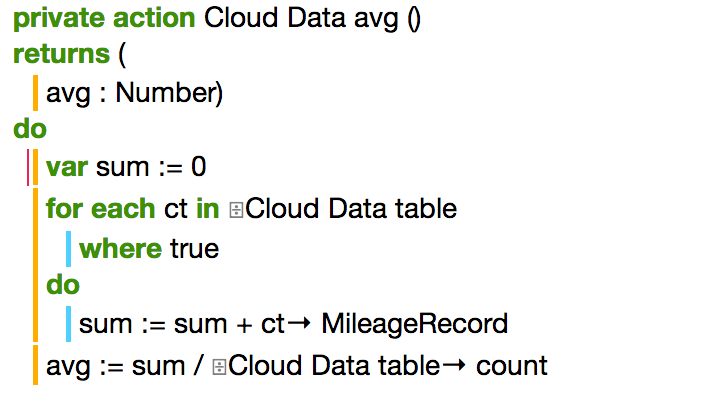
\includegraphics[width=250pt]{images/HelperFunction}
\nocaptionrule
\caption{custom function to provide avg functionality}
\label{fig:CloudTable_avg_fun}
\end{figure}

\subsubsection{Unsupported Language Features}
\label{sec:unsupportedLanguageFeatures}
There were some transformations that we were unable to perform due to limitations of the TouchDevelop language.  Local data structures, in our case the \NC{} data structure, can be passed as an input parameter (argument) or output parameter (return value) of a TouchDevelop action.  Due to language constraints, cloud data tables must be declared as global variables and cannot be used as input or output parameters.  \tool does not attempt to perform transformation in these situations.  In the future, a transformation could potentially be developed that would transform the local structure from a parameter to a global variable, and then the local to cloud data transformation could be performed.

 \NC{}s can be assigned to a variable using the assignment operator.  However, cloud data tables are able to be assigned due to their global nature.  We are therefore unable to transform any occurrences of a data collection that use the assignment operator. 

\tool also does not support the custom function transformation of \texttt{add many}.  We believe that this function could be implemented but it remains as future work.  For this reason,  \tool is unable to support transformations that involve the \texttt{add many} action.



\section{Evaluation}
\label{sec:evaluation}
To determine if \tool is useful we ask the following research questions.\\
Q1:  \textbf{APPLICABILITY}:  How applicable is the refactoring?\\
Q2:  \textbf{EFFORT}: How much effort is saved by \tool when refactoring?\\
Q3:  \textbf{ACCURACY}: How accurate is \tool when performing a refactoring ?\\
 
\subsection{Methodology}

To create a corpus, we wrote queries against a database of all publicly available scripts in the \TD script bazaar. We wanted to collect popular and mature scripts. 
Thus, our query returned top scripts (based on the number of times that each script was executed\TODO{verify that this is what ``number of runs'' means}) 
that contained a \NC{}. We retained the top \numScripts scripts.

%We also required the \NC{} be a global variable since 
%Our refactoring works on non-global variables, but using global variables simplifies the automated identification of refactoring targets. 

We ran the refactoring in batch mode. From each script in our corpus, our tool randomly selects one \NC{} as the target for refactoring. 

In order to determine the applicability of \tool, we report the number of scripts that our tool was able to refactor successfully, as well as the number of each kind of transformations performed inside a refactoring.



In order to determine the effort saved by using this refactoring tool we record the number of seconds each refactoring took. 



In order to validate the accuracy of \tool, we randomly chose \numManual scripts from the corpus of \numScripts refactored scripts. We ran the scripts and exercised the features for three minutes before and after each refactoring to ensure that the refactorings did not change the scripts' runtime behavior. Indeed, we did not observe any runtime differences before and after the refactoring. 

In addition to running these \numManual scripts we also carefully inspected the refactored code. We counted transformations that \tool
(i) applied correctly, (ii) applied incorrectly, and (iii) missed. We first manually created a set of transformations required for each refactoring, which we define as the \emph{golden standard}. We define a {\it TruePositive} as a transformation that \tool identified and applied correctly, and it was a part of the golden standard. 
We define {\it FalsePositive} as a transformation that \tool applies to the code, but it is not part of the golden standard. In other words, \tool transformed code that should not have been transformed.
We define a {\it FalseNegative} as a transformation that \tool did not apply, but it is in the golden standard. In other words, \tool missed applying a needed transformation.
 
 Using these metrics we calculate precision and recall for \tool, using the standard definitions:
\[precision = \frac{|True Positive|}{|True Positive|+|False Positive|}\]

\[recall = \frac{|True Positive|}{|True Positive|+|False Negative|}\]



\subsection{Results}

Next we present the results for each of the three research questions.


\textbf{Applicability: } 
Table~\ref{table:totalScripts} shows the results for running \tool on \numScripts scripts. 
Out of the \numScripts scripts that \tool attempted to refactor, 102 (94\%) met the preconditions for the refactoring.

Only 7 scripts were unable to be refactored. Out of these, 4 scripts did not meet precondition \POne (the \NC{} was passed as an argument to a function), and 1 did not meet precondition \PTwo (\NC{} was assigned to a local variable). The remaining 2 scripts exposed a limitation of the current implementation of \tool (they were using a currently unsupported function, \code{add many}). 
Thus, we think that our refactoring is widely applicable to \TD scripts that contain the \NC{} data structure.  

\TODO{breakout into preconditions}
\begin{table}[htdp]
\begin{center}
\begin{tabular}{ll}
Total Scripts & \numScripts \\
Number Successfully Refactored & 102 \\
Unsupported Language Features & 7 \\
\end{tabular}
\nocaptionrule
\caption{Total Scripts Refactored}
\label{table:totalScripts}
\end{center}
\end{table}%

\textbf{EFFORT}:  
Table~\ref{table:avgTrans} shows the number of transformations performed per each refactoring. The first column tabulates the total number of 
transformations per refactoring. The next three columns show the type of these transformations (i.e., direct, indirect, and custom function). The last column shows the running time for each refactoring.

Each refactoring consisted on an average of almost 12 transformations.  The most common transformation was indirect transformations with 10  transformations on average for each script.

The last column shows the time in seconds.  On average each refactoring took a total of 9 seconds to complete.  The maximum length of time any single refactoring took was 18 seconds.  As the number of transformations on average was 12, this shows that our refactoring tool saves significant effort, as the time to make these transformations by hand would clearly exceed a few seconds.  

%TODO: move to results
%Table~\ref{table:avgTrans} shows  the refactoring times.  The longest refactoring took 18 seconds, but the median time was only 9 seconds.  The majority of the time spent doing the refactoring was spent locating transformations, so the time that the refactoring took was correlated with the program size, not with the number of transformations performed for each script.



\begin{table}[htdp]
\begin{center}
\begin{tabular}{lclclclclcl}
 & Total & Direct & Indirect & Custom & Time \\
  & Trans & Trans & Trans & Function & [secs] \\
  \hline
  \hline
AVG & 11.6 & 1.20 & 9.07 & 1.34 & 9.30 \\
\hline
MAX & 112 & 13 & 112 & 19 & 18 \\
\hline
\end{tabular}
\nocaptionrule
\caption{Average Transformations}
\end{center}
\label{table:avgTrans}
\end{table}%

\begin{figure}[htbp!]
\begin{center}
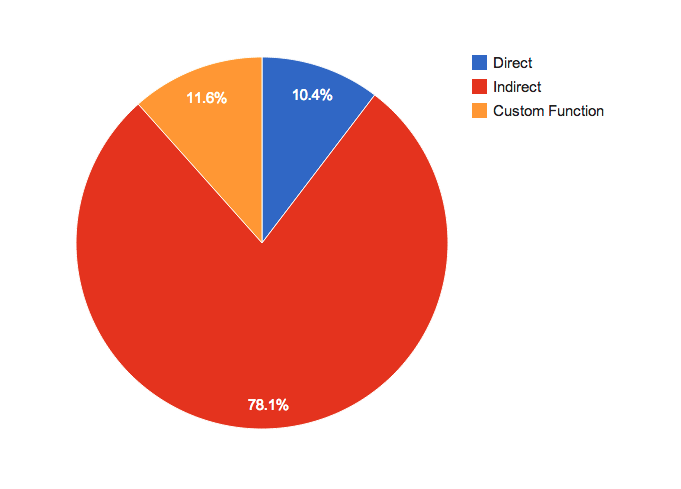
\includegraphics[width=250pt]{images/TransformationsChart}
\nocaptionrule
\caption{Transformations by Percentage}
\label{fig:transformations_pieChart}
\end{center}
\end{figure}

\textbf{ACCURACY}: By manually checking 20 scripts, we analyzed the precision and recall for our tool.  We found a precision of 100\%.  We also calculated the recall, and our recall value was 94\%. There were over 145 transformations that we inspected in these 20 scripts, and we only found 8 potential transformations that \tool missed.

\begin{table}[htdp]
\begin{center}
\begin{tabular}{ll}

Precision & 100\% \\
Recall & 95\% \\
\end{tabular}
\nocaptionrule
\caption{Precision and Recall values}
\end{center}
\label{table:precAndRecall}
\end{table}%

\subsection{Case Studies}

\subsubsection{Motivating Example}
We forked the Mileage Tracker script and created our own Mileage Tracker script. Without making any logical change to the script, we used \NC{} instead of number map to store data. We then manually replaced a slice api call with corresponding logic as the slice api call is not available with \NC{}. We ran both the original script and our manual changes to ensure that both scripts exhibited the exact same functionality. The new Mileage Tracker script is available in TouchDevelop with script id \texttt{mfbb}.  We then refactored the Mileage Tracker script using \tool. All the transformations were successfully applied and script did not have any compilation errors. Though to ensure that script behavior was exactly same as before we needed to make two lines of code change in InitializeApplicationSettings method of the script. As Microsoft TouchDevelop recent version removed is invalid with cloud data table, we have to replace it with corresponding logical step. The other one line of change in code is to enable everyone session on the cloud data table. This will allow multiple users with their own separate sessions to share same cloud data table. We ran the refactored Mileage Tracker application with three different devices, two laptops and one mobile phone to verify Mileage Tracker is indeed refactored into multi device, multi user application. Thus, with our automated refactorings and two lines of code changes we were successfully able to convert a single user, single device application into multi user, multi device application. The refactored Mileage Tracker Appliation is available in TouchDevelop with id \texttt{eyhca} and name Mileage Tracker Refactored. 

\subsubsection{BlockY World}
To further demonstrate the usefulness of cloud refactoring, we applied it on BlockY World, a game script written for TouchDevelop. The BlockY World script id is skdk. 65 users are following this game and the game has been installed 350.  To convert this game from single device to multi device/multi user game via refactoring, we used our tool to refactor all the collections to cloud data types. BlockY World has 8 \NC{}s and one \texttt{picture collection}. As TouchDevelop cloud data tables do not support picture type, we are unable to convert the picture collection to cloud data type.  All 8 \NC{}s were automatically refactored into corresponding cloud data type using the tool. We also added some manual code to initialize and share the data. 

However, we were unable to convert BlockY World into a multi device game.  We throughly analyzed the script to see what additional steps would be needed to complete the transition to a multiplayer game.

Our further analysis of BlockyWorld suggests that some global variables also need to be moved to cloud because to make the script multi device some global variables also need to be shared across devices over the cloud. For instance, variables like $old_x$ and $old_y$ and $curr_x$ and $curr_y$ needs to be stored across the devices. These variables are of type number.  

BlockY World consists of some variables whose cloud type representation is not available at this point of time. ercan is game board variable used for the BlockY World game. In order to effectively share the game board across multiple devices, we need to move variable ercan to cloud. Currently no cloud data type implementation supports game board variables. BlockyWorld consists many such variables whose cloud data type conversion is not possible.

We also determined that for this application, eventually consistency was not responsive enough for realtime gaming.  Though the eventual consistency model works fine with many types of applications, it is not particularly  suited for games where real time data needs to be shared quickly across device. TouchDevelop team is planning to support flush implementation for synchronization with stronger consistency model~\cite{burckhardt2012cloud}, where any changes in local data is immediately synchronized with cloud data, though it is not available currently. Though we are not able to refactor BlockY World into a multi device application through refactoring, analysis of BlockY World brought into light certain implementation level issues of both TouchDevelop as well as textsc{cloudifyer} that hinders widespread practical usage of textsc{cloudifyer} in case of realtime gaming application refactoring. 


\subsection{Threats to validity}
\textbf{Construct Validity:}  Does the evaluation of candidate scripts prove the applicability of our tool?  Since the refactoring to the cloud is such a new part of the TouchDevelop language, there is not a lot of data for us to identify when developers will actually choose to refactor to the cloud.  By showing that most of the scripts that use the local data structure are applicable candidates, we can show that there is wide applicability for our solution, should developers choose to use it or not.

\textbf{Internal Validity:}  We minimized the threat of internal validity by performing a case study of apps that were written before the introduction of Cloud Data, and by using publicly available scripts, the developers were unaware of our study.  

\textbf{External Validity:}  Do our results generalize? We chose over 100 of the most commonly run scripts to use as our corpus, but we put no restrictions on the tags, or types of the scripts.  Our selection include scripts tagged with entertainment,sports, games, education, productivity and platform bugs.  Since tags are not required in TouchDevelop we observed many scripts without tags.  However, in a addition to a wide variety of scripts tags, we also observed a variety of script types while performing the evaluations.  We do not foresee any reasons why these results would not generalize to all TouchDevelop scripts.

\textbf{Reliability:} Is our evaluation reliable? The scripts that we used to evaluate our tool are all available on the TouchDevelop website, and \tool is published on the TouchDevelop website with a script Id of //TODO FINAL VERSION OF SCRIPT ID.

Very few scripts in TouchDevelop have any tests at all.  We were not able to use these to verify that we did not break the runtime behavior of the scripts.  In order to mitigate this we manually validated a random selection of scripts to ensure constant runtime behavior before and after our refactoring.



\section{Related Work}
\label{sec:relatedWork}

Strauch et al.~\cite{strauchmigrating} provide a methodology for refactoring applications to move from application data to cloud data.  Their approach is based on finding a migration scenario that depends upon requirements and then mapping the scenario to one of their existing cloud data patterns. Though this paper provided a methodology at a high level, the actual application refactoring is completely manual and left up to programmers. Also, moving application data to the cloud was also manual  and programmer will have to be involved at multiple level to make this refactoring possible.  

Ling et al.~\cite{ling2010refactoring} provided a systematic refactoring approach using theoretic computing to formally define a mechanism to convert object oriented systems into service oriented architecture systems. The services then can be moved to the cloud to benefit from the elasticity of the cloud. Again, this approach leads to the use of manual refactoring and manual moving of services to cloud. 

\tool is different from both these approaches in that it performs the refactoring in an automated manner, thus saving programmers from the effort of moving data structures manually to the cloud.  

Kwon and Tilevich~\cite{kwon2013cloud} proposed \emph{Cloud Refactoring}, a tool to automatically refactor methods of an enterprise application system into services that can be then ported to the cloud. Their tool also determines if a method is a good candidate for refactoring via static analysis of code and dynamic traces generated using application execution. However, even though the methods are automatically refactored into services, they still must be moved to the cloud manually.  \tool performs the refactoring automatically, but also handles the transfer to the cloud.  We do believe that Kwon and Tilevich's approach is a big leap forward in right direction.  

CloudCone~\cite{chun2011clonecloud}, also attempts to harness the power of mobile cloud computing, but their approach is significantly different then ours in that they create clones on the cloud, and then move the execution of the application as well as it's state between the cloud and the device.

\section{Conclusions and Future Work}
\label{sec:conclusions}
In this paper we present \tool, a tool to refactor local data structures into cloud data structures.  We have shown that it is able to automatically transform most usages of \NC{} into cloud data references.  We are able to perform these transformations while still preserving the behavior of the application.  Should the user choose to take further advantage of the cloud data features, in some cases only a few lines of code are needed to take advantage of the cloud data features to provide more functionality. 

In the future, it would be nice to automate those changes, so in addition to being able to refactor their data to the cloud, we would like to provide an automated transformation tool that would enable multiuser features to be automatically added to scripts.




% We recommend abbrvnat bibliography style.

\bibliographystyle{abbrvnat}

% The bibliography should be embedded for final submission.

\bibliography{refs}


\end{document}

%                       Revision History
%                       -------- -------
%  Date         Person  Ver.    Change
%  ----         ------  ----    ------

%  2013.06.29   TU      0.1--4  comments on permission/copyright notices

